The CDF of $V$ is defined as 
\begin{align}
    F_V(v) &= \pr{V \le v} \\
           &= \pr{ -2 \ln(1-U)\le v} \\
           &= \pr{\ln(1-U) \ge -\frac{v}{2}}\\
           &= \pr{1-U \ge \exp\brak{-\frac{v}{2}}}\\
           &= \pr{U \le 1- \exp\brak{-\frac{v}{2}}}\\
           &= F_U\brak{1- \exp\brak{-\frac{v}{2}}}
%           &=  (1-(exp(-v/2))
\label{eq:probman_cdf_V_temp}
\end{align}
From \eqref{eq:probman_cdf_U},
\begin{align}
F_U(x) = 
\begin{cases}
0 &  x < 0 \\
x & 0 \le x \le 1 \\
1 & x > 1
\end{cases}
\end{align}
%
Substituting the above in \eqref{eq:probman_cdf_V_temp},
%
\begin{multline}
F_U\brak{1- \exp\brak{-\frac{v}{2}}} =
\\
\begin{cases}
0 &  1- \exp\brak{-\frac{v}{2}} < 0 \\
1- \exp\brak{-\frac{v}{2}} & 0 \le 1- \exp\brak{-\frac{v}{2}} \le 1 \\
1 & 1- \exp\brak{-\frac{v}{2}} > 1
\end{cases}
\end{multline}
%
After some algebra, the above conditions yield
\begin{align}
F_V(v) = 
\begin{cases}
0 & v < 0 \\
1- exp\brak{-\frac{v}{2}} & v \ge 0
\end{cases}
\label{eq:probman_V_cdf_anal}
\end{align}
%
which is the CDF of the exponential distribution with parameter $\frac{1}{2}$.  The following
code generates the CDF obtained using \eqref{eq:probman_V_cdf_sim} and \eqref{eq:probman_V_cdf_anal} in Fig. \ref{fig:probman_V_cdf_analsim}.
\begin{lstlisting}
codes/quantile/ASSIGNMENT_1.py
\end{lstlisting}
\begin{figure}[!ht]
\centering
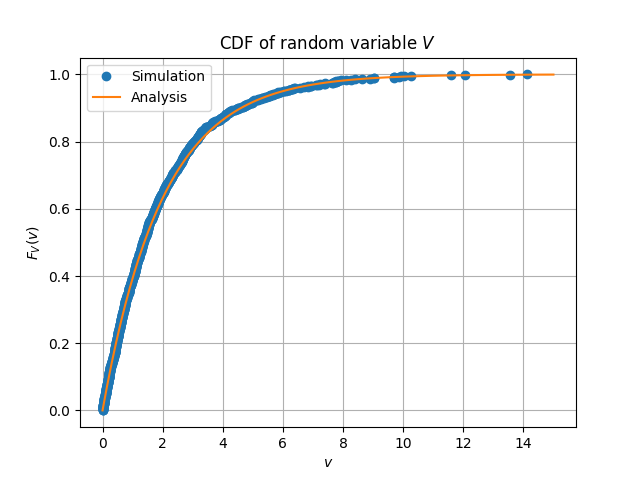
\includegraphics[width=\columnwidth]{figs/quantile/quantile.png}
\caption{}
\label{fig:probman_V_cdf_analsim}
\end{figure}
{\em Comment:}
For the uniform distribution, $0 < U < 1$.  For any random variable $V, 0 < F_V(x) < 1$.  This
similarity between $U$ and $F_V(x)$ is used to generate the random variable $V$ from $U$.
Thus,
\begin{align}
V = F_V^{-1}(U)
\end{align}
%
where $F_V^{-1}$ is defined to be a {\em quantile} function.
